\documentclass[12pt,a4paper,twoside]{book}
\usepackage{graphicx}
\usepackage{setspace}	%double spacing for text, single for captions, footnotes, etc.
%\usepackage{hypernat} 	%substitut de cite que permet fer hyperlinks
\usepackage[numbers]{natbib} % substituye a 'hypernat' que funciona en Windows.
\usepackage[spanish]{babel}
\usepackage[utf8]{inputenc}
\usepackage{color}
\usepackage{hhline} 		% extended styles for tables
\usepackage{multirow}
%\usepackage{subfigure}
\usepackage{fancyhdr}
\usepackage{acronym}
\usepackage{hyperref}
\usepackage{amsmath,amssymb}
\usepackage{epsfig, amsmath}
\usepackage{algorithm}
\usepackage{algorithmic}
\usepackage{subcaption} %For add subfigures

% general settings
\hypersetup{
	linktocpage=true,
	colorlinks=true,
	linkcolor=blue,
	citecolor=blue,
}
\definecolor{Hgray}{gray}{0.6}

\newenvironment{definition}[1][Definition]{\begin{trivlist}
\item[\hskip \labelsep {\bfseries #1}]}{\end{trivlist}}

\setlength{\topmargin}{0cm}
\setlength{\textheight}{23cm}
\setlength{\textwidth}{17cm}
\setlength{\oddsidemargin}{0cm}
\setlength{\evensidemargin}{0cm}
\setlength{\headheight}{1cm}

% indica que las 'sub-sub-sections' sean numeradas y aparezcan en el indice
\setcounter{secnumdepth}{3}
\setcounter{tocdepth}{2}

% settings for code
\renewcommand{\algorithmicrequire}{\textbf{Entrada: }}
\renewcommand{\algorithmicensure}{\textbf{Salida: }}

%%%%%%%%%%%%
% DOCUMENT %
%%%%%%%%%%%%
\begin{document}

% portada
\newpage
\thispagestyle{empty}

\baselineskip 2em

%\vspace*{1cm}

\centerline{
\includegraphics[width=0.6\textwidth]{images/UOC-logo}}
\begin{center}
\textsc{Universitat Oberta de Catalunya (UOC) \\
 Máster Universitario en Ciencia de Datos (\textit{Data Science})\\}

%\centerline {\pic{UOC}{4cm}}

\vspace*{1.5cm}

\textsc{\Large TRABAJO FINAL DE MÁSTER}

\vspace*{0.5cm}

\textsc{\large Área: 2}


%\textbf{\Huge VirtualTechLab Model: }

\vspace*{2.0cm}

\textbf{\Large CLASIFICADOR DOCUMENTOS MÉDICOS HOPE }

\vspace{2.5cm}
\baselineskip 1em

\baselineskip 2em
-----------------------------------------------------------------------------\\
Autor:      Rubén Vasallo Gonzalez \\
Profesor:   Jordi Casas Roma\\
Tutor:      Carlos Luis Sanchez Bocanegra\\
Co-Tutor:   Rafael Pastor Vargas\\
-----------------------------------------------------------------------------\\
\vspace*{1.5cm}
Barcelona, \today

\end{center}

\newpage
\pagestyle{empty}
\hfill

\newpage
% abstract
\pagenumbering{roman} 
\setcounter{page}{1} 
\pagestyle{plain}

%%%%%%%%%%%%%%%%
%%% CREDITOS %%%
%%%%%%%%%%%%%%%%
\chapter*{Créditos/Copyright}

\vspace{1cm}

\begin{figure}[ht]
    \centering
	
\includegraphics[scale=1]{images/license.png}
\end{figure}

Esta obra está sujeta a una licencia de Reconocimiento -  NoComercial - SinObraDerivada

\href{https://creativecommons.org/licenses/by-nc-nd/3.0/es/}{3.0 España de CreativeCommons}.

%%%%%%%%%%%%%
%%% FICHA %%%
%%%%%%%%%%%%%
\chapter*{FICHA DEL TRABAJO FINAL}

\begin{table}[ht]
	\centering{}
	\renewcommand{\arraystretch}{2}
	\begin{tabular}{r | l}
		\hline
		Título del trabajo: & CLASIFICADOR DOCUMENTOS MÉDICOS HOPE\\
		\hline
        Nombre del autor: & Rubén Vasallo Gonzalez\\
		\hline
        Nombre del colaborador/a docente: & Carlos Luis Sanchez Bocanegra, Rafael Pastor Vargas \\
		\hline
        Nombre del PRA: & Jordi Casas Roma \\
		\hline
        Fecha de entrega (mm/aaaa): & 01/2021\\
		\hline
        Titulación o programa: & Máster Universitario en Ciencia de Datos\\
		\hline
        Área del Trabajo Final: & M2.979 - TFM\\
		\hline
        Idioma del trabajo: & Español\\
		\hline
        Palabras clave & hope, clasificador, medicina\\
		\hline
	\end{tabular}
\end{table}

%%%%%%%%%%%%%%%%%%%
%%% DEDICATORIA %%%
%%%%%%%%%%%%%%%%%%%
\chapter*{Dedicatoria/Cita}

Quiero dedicarle este trabajo a mis mentores \textit{Carlos Luis Sanchez Bocanegra} y \textit{Rafael Pastor Vargas} que me han ayudado, apoyado y guiado en todo momento para conseguir los objetivos del máster.

%%%%%%%%%%%%%%%%%%%
%%% Agradecimientos %%%
%%%%%%%%%%%%%%%%%%%
\chapter*{Agradecimientos}

\paragraph{}
Quiero agradecer a \textit{Carlos Luis Sanchez Bocanegra} por invitarme participar en el Proyecto HOPE y poder aportar mi granito de arena a este gran proyecto.

\paragraph{}
También quiero dar la gracias a todos los miembros del proyecto HOPE que me han dado la bienvenida al grupo y me han facilitado la vida en unas circunstancias en las que, cuando entre en este, no eran las más idóneas. La mayoría de integrantes del grupo son médicos y la saturación de trabajo que había por el COVID-19 era enorme. Tengo claro que sin ellos y sin la ayuda en especial de Carlos y \textit{Nicolas Passadore} que ha estado luchando para conseguir un dataset con más observaciones, este Máster no habría sido posible.

%%%%%%%%%%%%%%%%
%%% RESUMEN  %%%
%%%%%%%%%%%%%%%%
\chapter*{Abstract}
\addcontentsline{toc}{chapter}{Abstract}

\onehalfspacing
\paragraph{}
This Final Master's Thesis {\textit{FMT}} was born from the need to be able to have in a simple, up-to-date and immediate way, medical bibliographic references cataloged according to the information and the patient's symptoms, being able to make a ranking of more or less interest function of the feedback provided by health professionals on these bibliographic references.

\paragraph{}
\textbf{Resumen}:
\paragraph{}
Este Trabajo de Final de Máster (\textit{TFM}) nace de la necesidad de poder disponer de una manera sencilla, actualizada e inmediata, referencias bibliográficas médicas catalogadas según la información y los síntomas que tienen del paciente, pudiendo hacer una clasificación (\textit{ranking}) de más o menos interés en función de la valoración (\textit{feedback}) aportada por los profesionales sanitarios sobre estas referencias bibliográficas.

\vspace{1.5cm}

\textbf{Palabras clave}: hope, clasificador, artículos, médicos, PCA, KNN, Regresión Logística, logit, Random Forest, SVM
\newpage

\pagestyle{fancy}
\renewcommand{\chaptermark}[1]{ \markboth{#1}{}}
\renewcommand{\sectionmark}[1]{\markright{ \thesection.\ #1}}
\lhead[\fancyplain{}{\bfseries\thepage}]{\fancyplain{}{\bfseries\rightmark}}
\rhead[\fancyplain{}{\bfseries\leftmark}]{\fancyplain{}{\bfseries\thepage}}
\cfoot{}

% indice
\cleardoublepage
\phantomsection
\addcontentsline{toc}{chapter}{Índice}
\tableofcontents
% listado de figuras
\cleardoublepage
\phantomsection
\addcontentsline{toc}{chapter}{Listado de Figuras}
\listoffigures
% listado de tablas
\cleardoublepage
\phantomsection
\addcontentsline{toc}{chapter}{Listado de Tablas}
\listoftables

\thispagestyle{empty}

\pagenumbering{arabic}

\pagestyle{fancy}
\renewcommand{\chaptermark}[1]{ \markboth{#1}{}}
\renewcommand{\sectionmark}[1]{\markright{ \thesection.\ #1}}
\lhead[\fancyplain{}{\bfseries\thepage}]{\fancyplain{}{\bfseries\rightmark}}
\rhead[\fancyplain{}{\bfseries\leftmark}]{\fancyplain{}{\bfseries\thepage}}
\cfoot{}

\onehalfspacing

% capitulos del documento
\chapter{Introducción}
\label{chapter:introduccion}


%%% SECTION
\section{Descripción general del problema}
\label{def:def1}

\paragraph{}
El Trabajo de Final de Máster (\textit{TFM}) que aquí se presenta nace de la necesidad por parte de los profesionales sanitarios de poder tener la información más exacta posible sobre las mejores referencias bibliográficas actuales sobre tratamientos a aplicar a un paciente, dado unos síntomas concretos. Actualmente existe infinidad de referencias medicas que los profesionales sanitarios pueden consultar, pero esta información es tan abundante que acaba siendo engorrosa de consultar. Esto hace que, muchas veces sea complicado encontrar la información sobre estas referencias bibliográficas para tratar algunas enfermedades. En el ámbito de la medicina el tiempo perdido puede costar vidas y es un precio demasiado elevado a pagar, tanto a nivel económico como emocional.

\paragraph{}
Los profesionales sanitarios necesitan poder disponer de una plataforma que sea capaz de poder facilitarles estas referencias bibliográficas actuales lo más exactas y personalizadas que sean posible, ajustándose a la búsqueda de la información que poseen de sus pacientes.

\paragraph{}
Bajo esa premisa nace el proyecto HOPE (que significa \textit{Health Operations for Personalized Evidence} en ingles) con el objetivo de ayudar a estos profesionales sanitarios a encontrar estas referencias bibliográficas que necesitan de la manera más rápida y fácil posible. Actualmente existen bases de datos de confianza en donde los profesionales sanitarios y el publico en general puede buscar estas referencias de ensayos y estudios clínicos con información fiable y desarrollados con anterioridad, pero no siempre es fácil o rápido encontrar estos resultados.

\paragraph{}
El proyecto HOPE es un sistema basado en inteligencia artificial para identificar la información de casos clínicos registrados en la Historia Clínica Electrónica, en base a los cuales realiza una búsqueda única por paciente para proporcionar al profesional sanitario recomendaciones de referencias bibliográficas donde constan tratamientos, estudios de investigación e información para ayudar al paciente. Todo en base a registros de fuentes científicas de información. En este proyecto, los profesionales sanitarios de todo el mundo puede consultar en una base de datos estas referencias y ver que otros tratamientos relacionados con los síntomas de sus pacientes han dado resultado. Todo y con eso, el sistema no siempre devuelve las referencias actuales más relevantes por lo que, no siempre la información consultada es útil.

\paragraph{}
Ademas, actualmente los profesionales sanitarios pueden valorar si la información recibida ha sido útil o no respecto a la búsqueda que han realizado, por lo que con esta valoración (\textit{feedback}), se pretende mejorar el sistema actual complementándolo con un modelo clasificador capaz de ayudar al actual a entregar realmente las referencias que son más útiles basándose en la valoración que los profesionales sanitarios dan al sistema.

\paragraph{}
Este Trabajo de final de máster (\textit{TFM}) pretende ayudar a mejorar el proyecto HOPE, mejorando su algoritmo de Inteligencia Artificial para que los resultados se ajusten a las necesidades de información que requieren los profesionales sanitarios, en base a las búsquedas personalizadas que puedan hacer respecto a la información que tienen de sus pacientes. Para hacer esto se realizara un estudio de aproximación a conocer cual es el mejor modelo predictivo que puede ayudar a devolver esa información lo más exacta posible.

\section{Motivación personal}

\paragraph{}
En los duros tiempos en los que estamos viviendo actualmente, tanto económica como emocionalmente, es grato ver como la humanidad es capaz de dejar a un lado sus diferencias y unirse para afrontar problemas comunes. En el caso del proyecto HOPE, lo que más me atrajo fue la oportunidad de poder ayudar a encontrar soluciones a enfermedades que ya están en el último paso (o como médicamente se le describe, en cuidados paliativos).

\paragraph{}
Es evidente que este proyecto no va a dar una solución para curar cualquier enfermedad, pero si puede ayudar a los profesionales sanitarios a poder encontrar posibles soluciones a enfermedades complejas, ayudando a estos profesionales a buscar en la infinidad de documentación medica que existe, el tratamiento que más pueda ayudar a paliar o, quien sabe, curar una enfermedad que ya se daba por incurable. Esto mismo es lo que me motiva y mucho el poder ayudar ante estas situaciones.

\paragraph{}
También me ha motivado muchísimo el conocer a gente profesional que, independientemente del país al que pertenece o la profesión que tiene, se una al proyecto HOPE para participar y ayudar con sus conocimientos a hacer de este mundo, un lugar un poco mejor en el que vivir. Esta experiencia me esta enriqueciendo muchísimo personalmente y espero poder seguir contribuyendo al proyecto cuando este máster acabe.

\newpage
\chapter{Objetivos del Máster}
\label{chapter:objetivos}


\section{Objetivo principal}

\label{op:OP1}
\paragraph{OP1} - Poder recomendar al profesional sanitario las referencias bibliográficas actuales útiles y personalizadas, que refuerce las tomas de decisiones en base a la información que se dispone de este, pudiendo realizar una clasificación (\textit{ranking}) de más interés a menos.

\section{Objetivos secundarios}

\paragraph{}
Para poder cumplir con el objetivo principal \hyperref[op:OP1]{OP1}, desglosaremos los siguientes objetivos secundarios:

\label{os:OS1}
\paragraph{OS1} - Extraer la información de la base de datos y tratarla para quedarnos solo con la que consideramos valida.

\label{os:OS2}
\paragraph{OS2} - Hacer un análisis de componentes principales para poder seleccionar los atributos mas relevantes que influyen en los síntomas del paciente (estudio de que atributos son relevantes para alcanzar el objetivo).

\label{os:OS3}
\paragraph{OS3} - Enriquecer de los datos (\textit{data augmentation}) prediciendo los resultados que no están indicados si son relevantes. Aproximación por Vecinos más próximos (\textit{K-Nearest-Neighbor}).

\label{os:OS4}
\paragraph{OS4} - Predecir los resultados usando el algoritmo de aprendizaje supervisado para clasificación llamado Regresión logística '\textit{Logistic regression (logit)}'.

\label{os:OS5}
\paragraph{OS5} - Predecir los resultados usando el algoritmo de aprendizaje supervisado para clasificación llamado Bosques Aleatorios '\textit{Random Forests}'.

\label{os:OS6}
\paragraph{OS6} - Predecir los resultados usando el algoritmo de aprendizaje supervisado para clasificación llamado Máquinas de vector soporte '\textit{Support Vector Machines}'.

\label{os:OS7}
\paragraph{OS7} - Comparar los resultados obtenidos de los 3 modelos.
\newpage
\chapter{Planificación}
\label{chapter:planificación}


\section{Fechas importantes}

\paragraph{}
A continuación se detalla en la tabla \ref{table:gant_tabla} las fechas clave del proyecto.

\begin{table}[h!]
	\centering{}
	\begin{tabular}{ l | c | c | r }
		\hline
		Nombre & Fecha de inicio & Fecha de fin & Duración \\
		\hline
		\hline
		Reunión inicial con el cliente & 22/09/20 & 22/09/20 & 1  \\
		\hline
		Redacción de objetivos & 23/09/20 & 27/09/20 & 5  \\
		\hline
		Análisis de mercado & 28/09/20 & 18/10/20 & 21  \\
		\hline
		Enriquecer el DataSet & 19/10/20 & 01/11/20 & 14 \\
		\hline
		Diseño del Modelo 1 & 02/11/20 & 15/11/20 & 14  \\
		\hline
		Diseño del Modelo 2 & 16/11/20 & 29/11/20 & 14  \\
		\hline
		Diseño del Modelo 3 & 30/11/20 & 13/12/20 & 14  \\
		\hline
		Redacción de conclusiones & 14/12/20 & 27/12/20 & 14  \\
		\hline
		Preparación de la Defensa & 28/12/20 & 01/01/21 & 5  \\
		\hline
	\end{tabular}
	\caption{\textit{Tabla de fechas clave del proyecto}.}
	\label{table:gant_tabla}
\end{table}

\section{Diagrama Gantt}

\paragraph{}

A continuación se muestra en la figura \ref{fig:gant} el diagrama Gantt del proyecto.

\begin{figure}[h!]
	\centering
	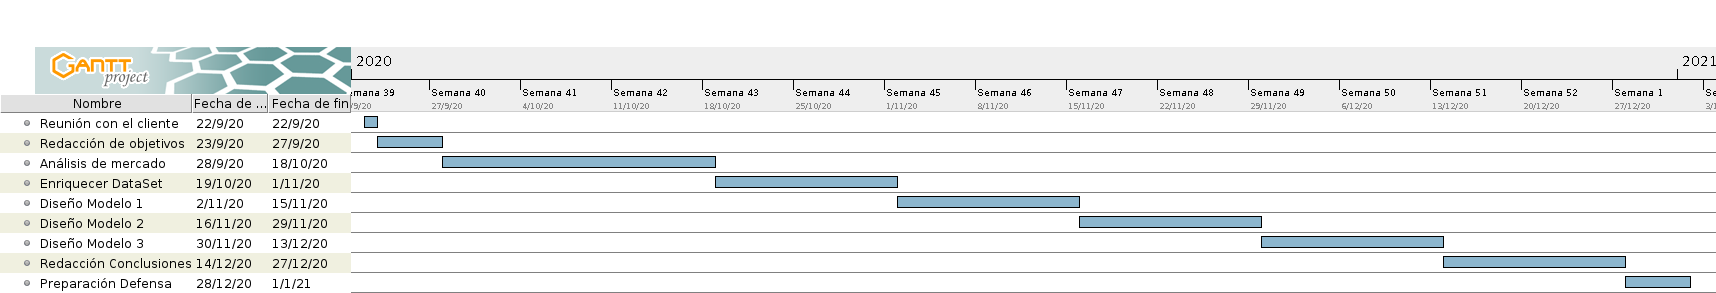
\includegraphics[width=0.9\textwidth]{figs/gant.png}
	\caption{Gantt del proyecto.}
	\label{fig:gant}
\end{figure}
\newpage
\chapter{Metodología}
\label{chapter:metodologia}


\section{Reuniones con el cliente}

\paragraph{}
Para poder comprender y abordar con éxito el \hyperref[op:OP1]{objetivo principal} se ha realizado dos reuniones en donde el cliente expuso el \hyperref[op:OP1]{problema} a abordar y el origen de los datos para poder realizar el estudio.

\paragraph{}
En estas reuniones se pudo observar que los datos facilitados por el usuario requerían de una limpieza y tratamiento para poder cumplir el objetivo principal, ya que muchas observaciones tenían información poco relevante que podía generar ruido.

\section{Limitaciones detectadas}

\paragraph{}
Realizando un primer análisis visual, se detecto que los datos aportados por el cliente eran insuficientes para completar el \hyperref[op:OP1]{OP1}, ya que solo se disponía de la información respecto de si una referencia bibliográfica había sido útil o no, pero no se disponía de la información suficientemente detallada para saber si había sido muy útil o poco útil para poder llegar a realizar una clasificación (\textit{ranking}). El cliente nos comenta que en el momento actual no dispone de ese nivel de detalle.

\paragraph{}
Se acuerda con el cliente que intentara conseguir más volumen de información y con más detalle para poder realizar la clasificación (\textit{ranking}) que necesita. Todo y con eso, se comenta que se realizara una aproximación para indicar si una referencia bibliográfica es útil o no dejando para mas adelante la opción de poder realizar la clasificación (\textit{ranking}) si se consigue ese nivel de detalle por parte del cliente.

\paragraph{}
También se pudo comprobar que el cliente disponía de un volumen de observaciones bajo por lo que se planteo la posibilidad de, o intentar obtener más observaciones facilitadas por el cliente, o intentar enriquecer las observaciones actuales generando nuevos datos por aproximación a los reales.

\paragraph{}
Finalmente se decidió estudiar si era viable generar nuevos valores por aproximación, debido a que en el momento en que se trato el problema, el cliente no podía facilitar más datos. Si a lo largo del estudio, el cliente conseguía obtener nuevas observaciones, estas serian añadidas al estudio para aproximar mejor la solución final.

\section{Análisis de datos}
\label{section:analisis_datos}

\paragraph{}
Tras recibir los datos por parte del cliente y realizar el primer análisis superficial, se detecto que el volumen de datos no era suficiente como para que los resultados que pudieran surgir del estudio, fueran concluyentes. Todo y con eso se acordó (tal y como se refleja en el \hyperref[os:OS1]{OS1}) hacer una valoración de los datos para ver si se podrían enriquecer de algún modo, mientras el cliente intenta obtener más volumen de datos.

\paragraph{}
Para ello, transformamos los datos que se nos facilito desde una base de datos donde se encontraba la información guardada en formato json, a un formato columnar en el que poder aplicar los modelos predictivos. Una vez tenemos los datos transformados, observamos que existen ciertos atributos que contienen listas de opciones como son los atributos \textit{pubmed\_keys} (que corresponde a las palabras clave que la API\cite{ref:pubmed_api} de pubmed nos devuelve para esta observación), \textit{articles} (que corresponde a los ids de los artículos relacionados con esa observación), \textit{articlesRevisedYear} y \textit{articlesRevisedMonth} (que corresponde a los años y meses de los artículos según están ordenados en el atributo \textit{articles}). Para poder recomendar artículos útiles, necesitamos tener una observación por artículo, para poder analizar posteriormente de manera independiente si ese artículo fue útil o no para la observación a la que hace referencia, por lo que aplicaremos las transformaciones necesarias para acabar obteniendo la representación de un artículo con su correspondiente \textit{feedback} por parte de los profesionales sanitarios. Todos los pasos para realizar las transformaciones se pueden consultar en el anexo (\nameref{anx01:procesado_datos}).

\paragraph{}
Aplicados las transformaciones anteriores, nos quedan los siguientes atributos que describimos a continuación:

\paragraph{• pedido.data.attributes.age:} Nos indica la edad del paciente en formato numérico (ejemplos de valores $=>$ 75,86,40,...).
\paragraph{• pedido.data.attributes.diagnostic\_main:} Nos indica el diagnostico principal que dio el profesional sanitario para la enfermedad que tiene el paciente en formato texto (ejemplos de valores $=>$ \textit{Fistula Peritoneal, Insuficiencia Respiratoria},...).
\paragraph{• pedido.data.attributes.gender:} Nos indica el sexo del paciente en formato texto (ejemplo de valor $=>$ \textit{male}).
\paragraph{• artículo:} Nos indica el identificador del artículo relacionado con el diagnostico principal en formato numérico (ejemplos de valores $=>$ 28694230,28805236,...).
\paragraph{• respuesta.articlesRevisedYear:} Nos indica el año de revisión del artículo referenciado por el identificador del campo artículo en formato numérico (ejemplos de valores $=>$ 2018,2017,2016,...).
\paragraph{• respuesta.articlesRevisedMonth:} Nos indica el mes de revisión del artículo referenciado por el identificador del campo artículo en formato numérico (ejemplos de valores $=>$ 4,12,6,9,...).
\paragraph{• respuesta.pubmed\_keys:} Nos indica las palabras clave relacionadas con el artículo del campo artículo en formato texto (ejemplos de valores $=>$ \textit{'Abdomen, Adenocarcinoma, Antiemetics, Blood', 'Abdomen, Analgesics, Bone, Catharsis', 'Abdomen, Anti-Bacterial Agents, Diuresis'},...).
\label{section:analisis_datos_utilidad}
\paragraph{• utilidad:} Nos indica si un profesional sanitario ha considerado si el artículo referenciado en el campo artículo es útil para el diagnostico principal relacionado con la enfermedad del paciente. Este campo puede tener 3 valores: 1 para saber que el artículo es útil, 0 para indicar que no es útil y null para indicar que aun no se ha valorado.
\section{Análisis de componentes principales}
\label{section:pca}

\paragraph{}
El análisis de componentes principales (o como se le conoce en ingles por '\textit{Principal Component Analysis}' o \textit{PCA}), es un componente fundamental en el análisis de los datos, ya que permite reducir el número de atributos de un conjunto de datos para eliminar el ruido que los posteriores análisis/modelos predictivos funcionen con mejor precisión\cite{ref:pca_def}.

\paragraph{}
Por poner un ejemplo sencillo, imaginemos que tenemos un conjunto de datos de modelos de coche con muchísimos atributos de estos, como por ejemplo, el nombre del modelo, el color, el número de puertas, la cilindrada y la potencia, entre otros. Probablemente si intentáramos analizar los datos en busca de cual es el modelos que menos consume y quisiéramos crear un modelo predictivo con este objetivo, podríamos observar a simple vista que tenemos atributos que no nos son necesarios y que generaría distracción (ruido) a la hora de conseguir nuestro objetivo, como es el caso del atributo color, o el nombre del modelo.

\paragraph{}
El \textit{PCA} nos ayudara a encontrar cuales son los atributos más significativos del conjunto de datos para conseguir predecir el atributo que queremos\cite{ref:pca_def}, que en el caso que nos toca, es el atributo '\textit{utilidad}'.

\paragraph{}
Es cierto que, en nuestro conjunto de datos, no tenemos un gran volumen de atributos, pero este proceso nos puede ayudar a eliminar atributos con poca relevancia, para así, poder simplificar el modelo predictivo final.

\label{section:pca_standar}
\paragraph{}
Para realizar el \textit{PCA} nos ayudaremos de la librería \textit{sklearn.decomposition} que ya nos ofrece implementada la lógica para ejecutarlo. Ademas realizaremos la transformación de todos los atributos de Categóricos (texto) a Continuos (números continuos). Este paso se realiza para que el \textit{PCA} pueda realizar operaciones matemáticas sobre los valores de las observaciones. A este proceso se le conoce como factorización (\textit{factorize}). 

\paragraph{}
También estandarizaremos los valores a un rango de entre 1 y -1. Esto se realiza para igualar la importancia de todos los atributos, ya que en el paso anterior, al realizar la factorización, se nos puede dar el caso de tener valores muy altos (por ejemplo, al factorizar un atributo con 100 valores diferentes, se nos dará casos de observaciones que en un atributo tienen el valor 100, que puede ser más alto que otros valores que no se han transformado). Al realizar el PCA, si no se hace esta estandarización de los datos, los valores más altos se les dará más peso, pero no por eso pueden ser relevantes. Por lo que es imperativo el realizar esta estandarización.

\paragraph{}
Para realizar el PCA se han seguido 3 estrategias, para valorar que impacto tiene las observaciones según el conjunto de datos a analizar. Hemos realizado 3 iteraciones con el siguiente conjunto de datos:

\paragraph{• 1: } El dataset completo con las transformaciones mencionadas en el apartado \nameref{section:analisis_datos}

\paragraph{• 2: } El mismo dataset de la anterior iteración pero cogiendo solo las observaciones que se ha informado el atributo utilidad.

\paragraph{• 3: } El mismo dataset realizado en la iteración 2 pero añadiendo el mes y año del articulo, eliminando los atributos \textit{gender} (ya que todas las observaciones tienen el mismo valor) y articulo (que solo representa un identificador de un articulo). Ademas se expande el atributo \textit{respuesta.pubmed\_keys} para que exista una observación por cada keyword.

\paragraph{}
Una vez realizado esa transformación ya podemos ejecutar el PCA. Todos los pasos para realizar el PCA se pueden consultar en el anexo (\nameref{anx02:pca1}) para la iteración 1, el anexo (\nameref{anx02:pca2}) para la iteración 2 y el anexo (\nameref{anx02:pca3}) para la iteración 3.
\section{Enriquecimiento de los datos.}
\label{section:knn}

\paragraph{}
Debido a que tenemos un conjunto de datos con poco volumen, se acuerda el intentar enriquecer los datos (\hyperref[os:OS3]{OS3}) con los conjuntos de datos que tenemos que no tienen informado el atributo a predecir.

\paragraph{}
Para realizar esta operación utilizaremos el algoritmo de Enrquicecimiento por Aproximación de Vecinos más próximos (conocido por K-Nearest-Neighbor o K-NN). Este Algoritmo pretende asociar si un registro pertenece a un conjunto de datos o a otro dependiendo de la aproximación de otros resultados de los que si se conoce su valor \cite{ref:knn_def}.

\paragraph{}
Para poder ejecutar el algoritmo de K-NN necesitamos realizar la transformación de todos los
atributos Categóricos (texto) a Continuos (números continuos) y estandarizar, igual que se realizo para el caso del \hyperref[section:pca_standar]{PCA}. Esto es debido a que el algoritmo necesita tener valores numéricos para poder trabajar con los datos\cite{ref:knn_scaling}. Con esta transformación ya podemos realizar operaciones matemáticas con el conjunto de datos.

\paragraph{}
Para realizar el K-NN se han seguido 2 estrategias, para valorar que impacto tiene las observaciones según el conjunto de datos a analizar. Hemos realizado 2 iteraciones con el siguiente conjunto de datos:

\paragraph{• 1: } El dataset completo con las transformaciones mencionadas en el apartado \nameref{section:analisis_datos} eliminando las observaciones que no tenían identificado el atributo edad.

\paragraph{• 2: } El mismo dataset realizado en la iteración 1 pero eliminando los atributos \textit{gender} (ya que todas las observaciones tienen el mismo valor) y artículo (que solo representa un identificador de un artículo). Ademas se expande el atributo \textit{respuesta.pubmed\_keys} para que exista una observación por cada keyword.

\paragraph{}
Una vez realizado esa transformación ya podemos ejecutar el K-NN. Todos los pasos para realizar el K-NN se pueden consultar en el anexo (\nameref{anx03:knn1}) para la iteración 1 y el anexo (\nameref{anx03:knn2}) para la iteración 2.
\newpage
\chapter{Resultados}
\label{chapter:resultados}

\section{Análisis de componentes principales}
\label{resultados:pca}

\subsection{Conjunto de datos completo}

\paragraph{}
Para este caso, cuando se ejecuto el \textit{PCA} con el conjunto de datos completo, nos mostró tal y como podemos ver en la figura \ref{pcaOneResult}, que \textbf{con solo 3 atributos}, el modelo es \textbf{capaz de explicar (predecir) el 95\% de las observaciones}.

\begin{figure}[!htb]
  \centering
    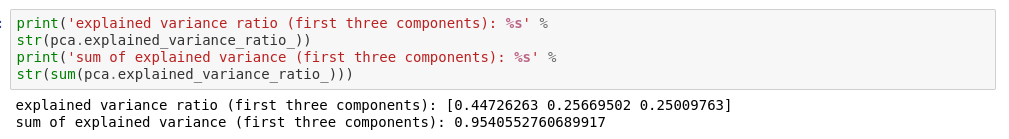
\includegraphics[width=0.9\textwidth]{images/resultados_procesado_de_datos_pca1_result.png}
    \caption{Resultado del \textit{PCA}.}
  \label{pcaOneResult}
\end{figure}

\paragraph{}
Dado que el \textit{PCA} solo nos muestra 3 atributos como relevantes, se pudo representar los resultados de las observaciones a un gráfico que mostramos en la figura \ref{pcaOneGraphic} dibujando los 3 componentes principales como si fueran 3 dimensiones, y pintando los valores a predecir sobre estos (aplicando el color rojo a las observaciones que catalogaron como no útiles, y azul los que catalogaron como útiles). En este gráfico pudimos observar que la gran mayoría de los puntos rojos se encontraban en el plano del componente principal 1 y 2, mientras que el azul estaba más repartido en los dos planos.

\begin{figure}[!htb]
  \centering
    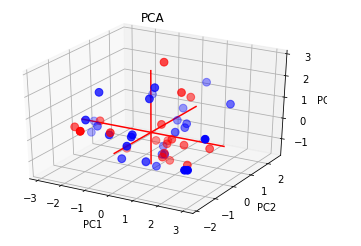
\includegraphics[width=0.4\textwidth]{images/resultados_procesado_de_datos_pca1_graphic.png}
    \caption{Proyección delos resultados del \textit{PCA} en una gráfica.}
  \label{pcaOneGraphic}
\end{figure}

\paragraph{}
A continuación, le pedimos al modelo que nos indicase cuales eran los 3 componentes que ha detectado que son los principales. Este nos mostró los resultados que se pueden ver en la figura \ref{pcaOneAtributos}. Para saber cuales son los componentes, tendremos que quedarnos para cada componente principal, el valor del atributo que más se acerque a 1.

\begin{figure}[!htb]
  \centering
    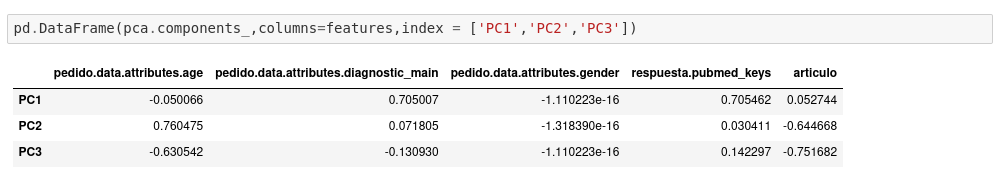
\includegraphics[width=0.9\textwidth]{images/resultados_procesado_de_datos_pca1_atributos.png}
    \caption{Proyección de los resultados del \textit{PCA} sobre los atributos del conjunto de datos.}
  \label{pcaOneAtributos}
\end{figure}

\paragraph{}
Para este caso, el \textit{PCA} nos mostró que \textbf{los 3 componentes principales son, el atributo \textit{pubmed\_keys}, el atributo \textit{age} y el atributo \textit{diagnostic\_main}}.

\subsection{Conjunto de datos añadiendo el mes y año del artículo y cogiendo solo las observaciones que se ha informado el atributo utilidad}
\label{result:pca_case2}
\paragraph{}
En este caso, el \textit{PCA} nos mostró tal y como podemos ver en la figura \ref{pcaTwoResult}, que se \textbf{necesita 5 atributos} para que el modelo sea \textbf{capaz de explicar (predecir) el 97\% de las observaciones}.

\begin{figure}[!htb]
  \centering
    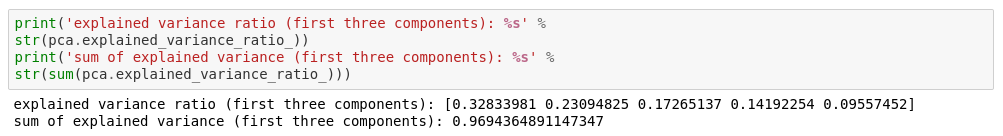
\includegraphics[width=0.9\textwidth]{images/resultados_procesado_de_datos_pca2_result.png}
    \caption{Resultado del \textit{PCA} de la segunda ejecución.}
  \label{pcaTwoResult}
\end{figure}

\paragraph{}
Para este caso, el \textit{PCA} nos mostró tal y como podemos ver en la figura \ref{pcaTwoAtributos}, que los \textbf{5 componentes principales} son, \textbf{el atributo \textit{diagnostic\_main}, el atributo \textit{Year}, el atributo \textit{pubmed\_keys}, el atributo \textit{age} y el atributo \textit{artículo}}.

\paragraph{}
La diferencia del número de atributos necesarios que nos muestra el \textit{PCA} respecto al conjunto anterior seguramente este debido a que el conjunto completo contiene un gran volumen de observaciones con el atributo '\textit{utilidad}' sin definir, lo que hace que prácticamente cualquier valor que tengan los atributos se acaben asociando a un resultado sin definir, como pasa en el conjunto de datos original. Al no tener en cuenta las observaciones con el atributo '\textit{utilidad}' sin definir, el \textit{PCA} ya nos indica que necesita analizar más atributos para acabar explicando el valor final.

\begin{figure}[!htb]
  \centering
    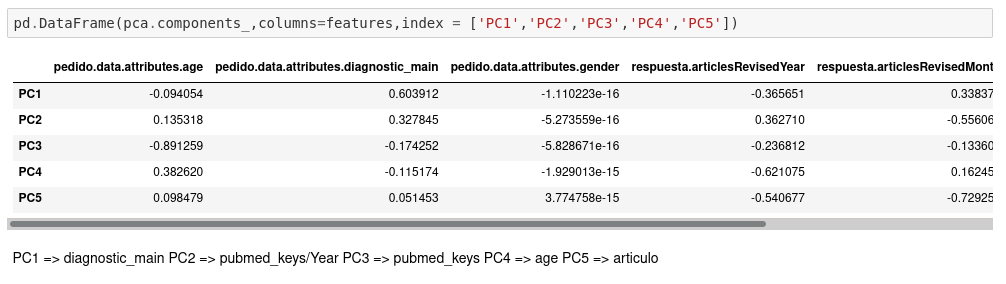
\includegraphics[width=0.9\textwidth]{images/resultados_procesado_de_datos_pca2_atributos.png}
    \caption{Proyección de los resultados del \textit{PCA} sobre los atributos del conjunto de datos para la segunda ejecución.}
  \label{pcaTwoAtributos}
\end{figure}

\subsection{Conjunto de datos solo con atributo utilidad definido, añadiendo el mes y año del artículo, eliminando los atributos \textit{gender} y artículo y expandiendo el atributo \textit{respuesta.pubmed\_keys}}
\label{result:pca_case3}
\paragraph{}
En este caso, el \textit{PCA} nos mostró tal y como podemos ver en la figura \ref{pcaThreeResult}, que se \textbf{necesita 4 atributos} para que el modelo sea \textbf{capaz de explicar (predecir) el 90\% de las observaciones}.

\begin{figure}[!htb]
  \centering
    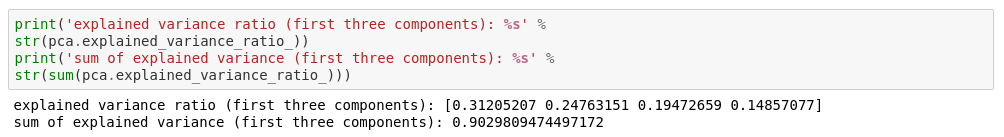
\includegraphics[width=0.9\textwidth]{images/resultados_procesado_de_datos_pca3_result.png}
    \caption{Resultado del \textit{PCA} de la tercera ejecución.}
  \label{pcaThreeResult}
\end{figure}

\paragraph{}
Para este caso, el \textit{PCA} nos mostró como podemos ver en la figura \ref{pcaThreeAtributos} , que los \textbf{4 componentes principales} son, \textbf{el atributo \textit{diagnostic\_main}, el atributo \textit{Month}, el atributo \textit{pubmed\_keys} y el atributo \textit{age}}.

\begin{figure}[!htb]
  \centering
    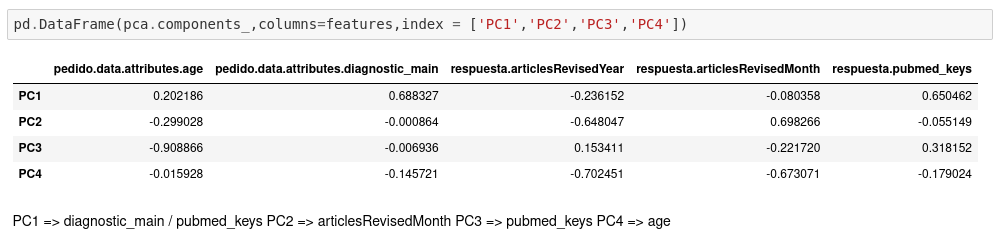
\includegraphics[width=0.9\textwidth]{images/resultados_procesado_de_datos_pca3_atributos.png}
    \caption{Proyección de los resultados del \textit{PCA} sobre los atributos del conjunto de datos para la tercera ejecución.}
  \label{pcaThreeAtributos}
\end{figure}

\section{Enriquecimiento de los datos. Aproximación por Vecinos más próximos (K-NN)}
\label{resultados:knn}

\subsection{Características de los conjuntos de datos a analizar}
\label{resultados:knn_caracteristicas}
Una vez realizado todas las transformaciones necesarias para poder ejecutar el algoritmo de \textit{K-NN} se pudo observar que tanto el '\textit{Conjunto de datos solo con atributo utilidad definido}' (Caso de estudio 1) como el '\textit{Conjunto de datos sólo con atributo utilidad definido, añadiendo el mes y año del artículo, eliminando los atributos gender y artículo y expandiendo el atributo respuesta.pubmed\_keys}' (Caso de estudio 2) \textbf{se observa el atributo a predecir (utilidad) sesgado}\cite{ref:sesgo} (no tienen un balanceo de datos equilibrado en el atributo a predecir), teniendo más resultados con valor 1 que con valor 0. Esto puede suponer que el modelo resultante tienda a estar sesgado\cite{ref:sesgo} hacia los resultados con valor 1 (debido a que tiene más datos en los que basarse para dar el resultado 1 frente a los otros datos como podemos ver en la figura \ref{knnDistUtilidad}.

\begin{figure}[!htb]
  \centering
    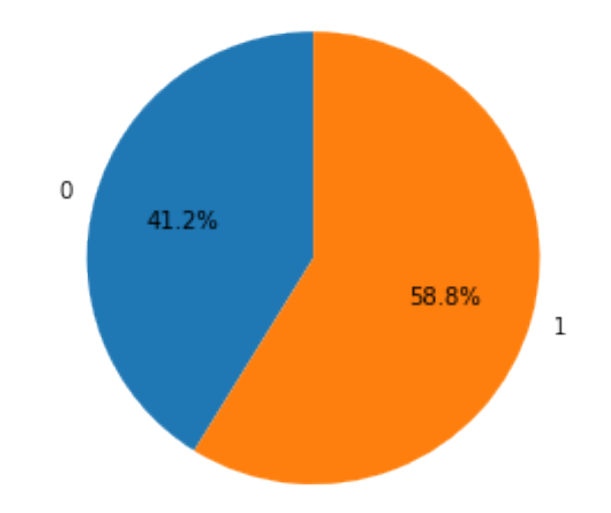
\includegraphics[width=0.3\textwidth]{images/resultados_knn_conjunto1.png}
    \caption{Distribución del atributo a predecir (utilidad) en el conjunto de entrenamiento.}
  \label{knnDistUtilidad}
\end{figure}

También, para el \textbf{caso de estudio 2}, se observo que la distribución del \textbf{atributo \textit{pubmed\_keys}}, una vez expandido, también \textbf{estaba sesgado} mostrando algunos resultados con pocas \textit{keywords} y otros como '\textit{Diuresis}' o '\textit{Abdomen}' con muchas observaciones como podemos ver en la figura \ref{knnDistKeywords}. Esto puede condicionar el comportamiento del modelo final igual que en el caso anterior, dando sospechas a que el modelo podría esta sobre ajustado\cite{ref:knn_overfiting}.

\begin{figure}[!htb]
  \centering
    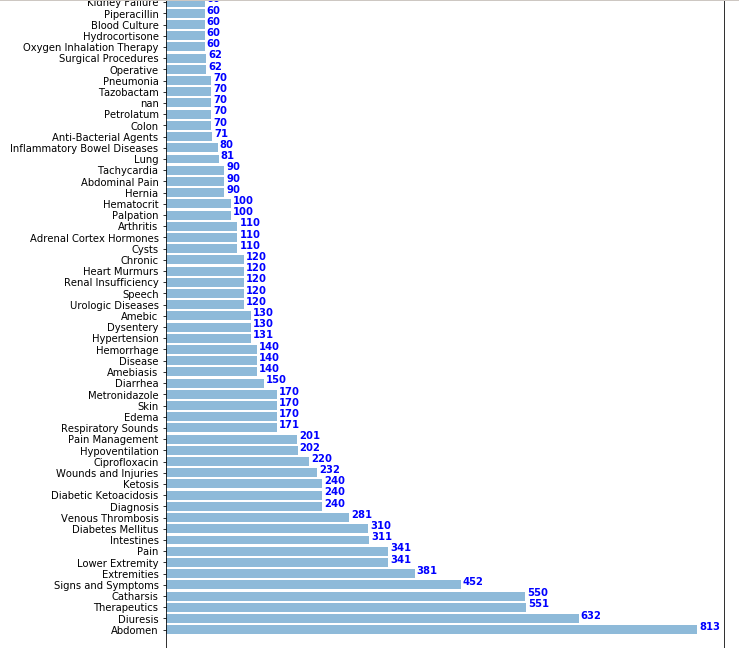
\includegraphics[width=0.8\textwidth]{images/resultados_knn_keywords.png}
    \caption{Distribución del atributo \textit{pubmed\_keys} en el conjunto de entrenamiento.}
  \label{knnDistKeywords}
\end{figure}

\paragraph{}
Finalmente, \textbf{para el entrenamiento y posterior validación} de los modelos nos ayudamos de la función '\textit{train\_test\_split}'\cite{ref:knn_train_test_split} del paquete '\textit{sklearn\.model\_selection}' que nos permite \textbf{dividir el conjunto de datos en dos grupos}, siendo el \textbf{primer grupo} para realizar el \textbf{entrenamiento} de los modelos que \textbf{corresponde al 75\% del total} de observaciones y el segundo grupo para realizar la \textbf{validación} de los modelos que \textbf{corresponde al 25\% del total} de observaciones.

\subsection{(Caso de estudio 1) Resultados del entrenamiento con el Conjunto de datos solo con atributo utilidad definido}

\paragraph{}
Antes de poder entrenar el algoritmo \textit{K-NN} fue necesario realizar un estudio para detectar a partir de que número de vecinos mas próximos (valor K), podemos dar por supuesto que el resultado esta relacionado con ellos. El algoritmo también nos permite poder decidir como calcular la distancia entre los vecinos (bien dando más relevancia a los vecinos con menos distancia '\textit{distance}'\cite{ref:knn_doc} o bien dando la misma relevancia a todos los vecinos que están próximos '\textit{uniform}'\cite{ref:knn_doc}).

Para realizar este estudio ejecutamos el modelo con diferentes valores de K y contrastamos que porcentaje de acierto tiene el modelo con un subconjunto del propio conjunto de datos que conocemos su valor final. Como podemos ver en la figura \ref{knnTrainCase1}, el valor más optimo de \textbf{K fue 6} utilizando el calculo de la distancia \textbf{'\textit{distance}'}, con un \textbf{porcentaje de acierto del 85\%}.

\paragraph{}
Si mostramos la matriz de confusión\cite{ref:confusion_matrix} (figura \ref{knnCMCase1}) para poder ver que porcentaje de aciertos tiene el modelo con el conjunto de test, se vio que tiene un porcentaje de aciertos bastante aceptable pese a tener más acierto para los casos con resultado 1 vrs. los resultados con valor 0 como comentamos anteriormente.

\begin{figure}[!htb]
    \begin{subfigure}[b]{0.45\linewidth}
    	\centering
	    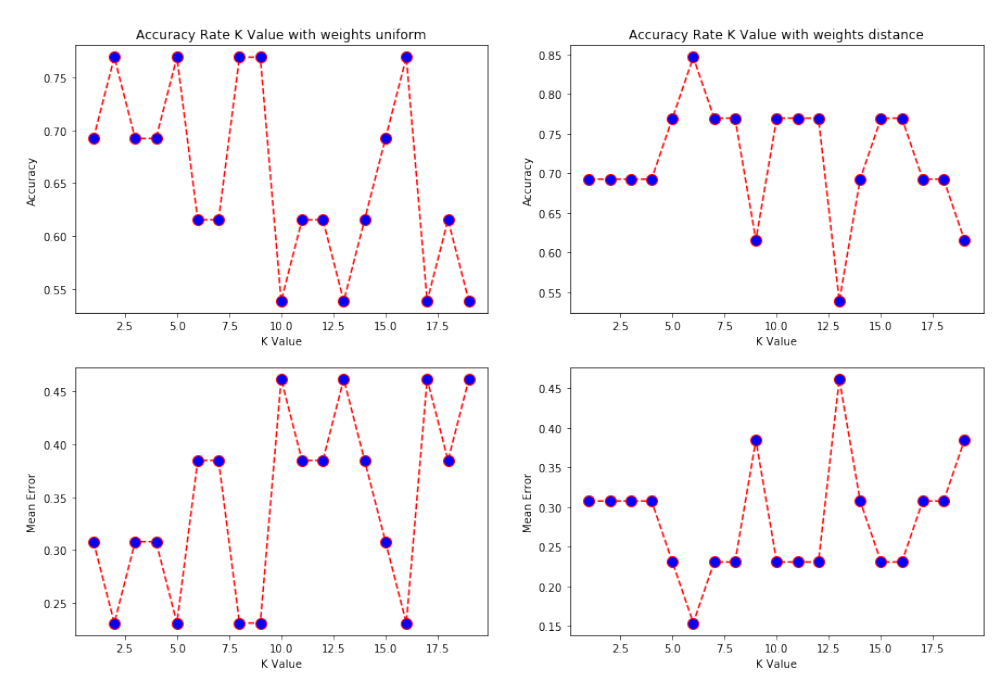
\includegraphics[width=0.9\textwidth]{images/resultados_knn_ent_conjunto1.png}
    	\caption{Calculo del valor K para el caso de estudio 1.}
		\label{knnTrainCase1}
	\end{subfigure}
	\begin{subfigure}[b]{0.45\linewidth} 
		\centering
		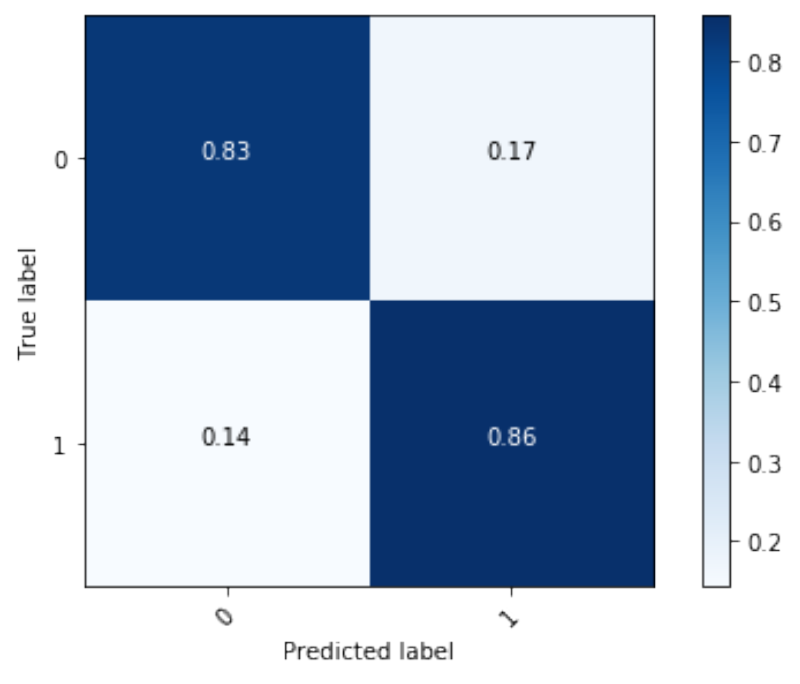
\includegraphics[width=0.7\textwidth]{images/resultados_knn_cm_conjunto1.png}
		\caption{Matriz de confusión para el modelo K-NN en el caso de estudio 1.}
		\label{knnCMCase1}
	\end{subfigure}
	\caption{Modelo K-NN en el caso de estudio 1.}
	\label{knnCase1}
\end{figure}

\subsection{(Caso de estudio 2) Conjunto de datos solo con atributo utilidad definido, añadiendo el mes y año del artículo, eliminando los atributos \textit{gender} y artículo y expandiendo el atributo \textit{respuesta.pubmed\_keys}}

\paragraph{}
Igual que en el caso anterior, se realizó el estudio para detectar a partir de que número de vecinos más próximos (valor K), podemos dar por supuesto que el resultado esta relacionado con ellos. A diferencia del caso anterior, podemos ver en la figura \ref{knnTrainCase2}, que el valor más optimo de \textbf{K fue 1} utilizando el calculo de la distancia \textbf{'\textit{uniform}'}, con un \textbf{porcentaje de acierto del 90\%}.

Si mostramos la matriz de confusión\cite{ref:confusion_matrix} (figura \ref{knnCMCase2}) para poder ver que porcentaje de aciertos tiene el modelo con el conjunto de test, vemos que tiene un porcentaje de aciertos bastante elevado por lo que podemos afirmar que \textbf{el modelo es sospechoso de estar sobre ajustado\cite{ref:knn_overfiting}}.

\begin{figure}[!htb]
    \begin{subfigure}[b]{0.45\linewidth}
    	\centering
	    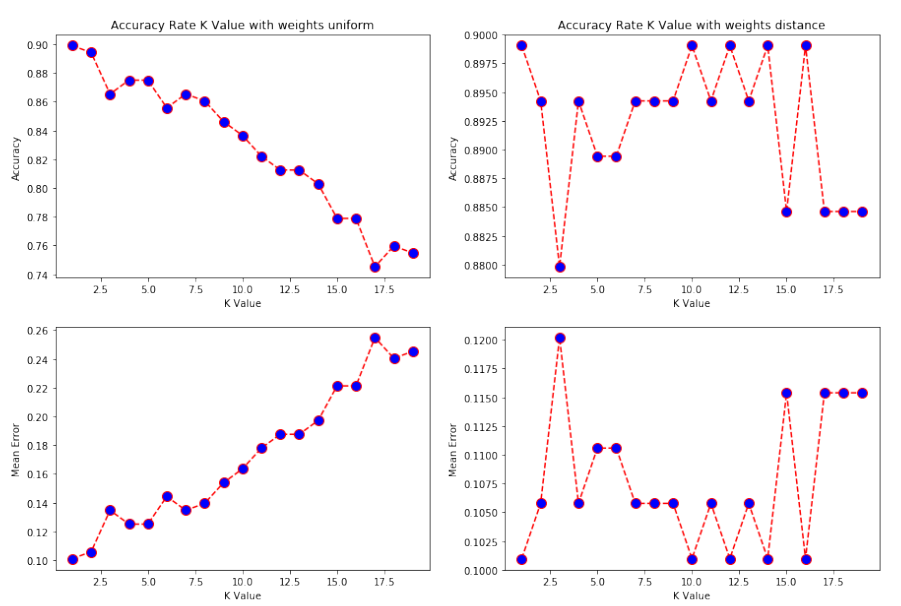
\includegraphics[width=0.9\textwidth]{images/resultados_knn_ent_conjunto2.png}
    	\caption{Calculo del valor K para el caso de estudio 2.}
		\label{knnTrainCase2}
	\end{subfigure}
	\begin{subfigure}[b]{0.45\linewidth} 
		\centering
		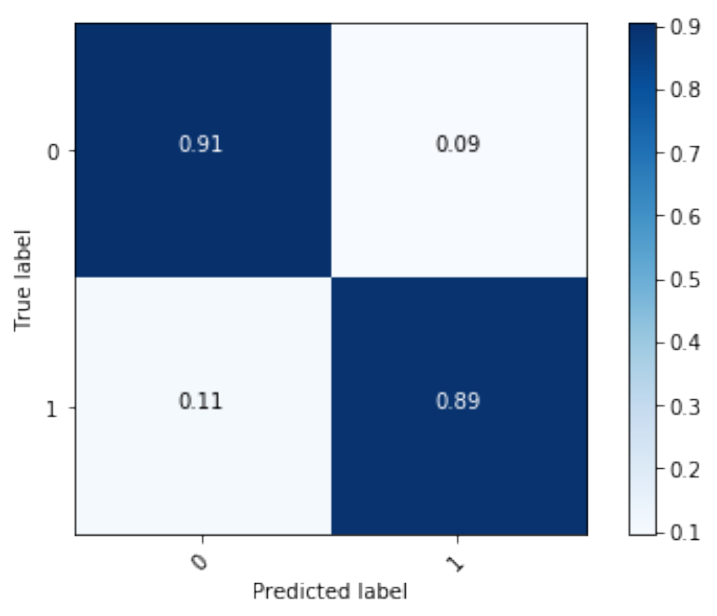
\includegraphics[width=0.7\textwidth]{images/resultados_knn_cm_conjunto2.png}
		\caption{Matriz de confusión para el modelo K-NN en el caso de estudio 2.}
		\label{knnCMCase2}
	\end{subfigure}
	\caption{Modelo K-NN en el caso de estudio 2.}
	\label{knnCase1}
\end{figure}

\subsection{Conclusiones del modelo K-NN}
\label{resultados:knn_conclusiones}

\paragraph{}
Pese a que aparentemente, el caso de estudio 1 tiene unos resultados aceptables, \textbf{aconsejamos} al cliente \textbf{no utilizar el algoritmo de \textit{K-NN}} para enriquecer los datos del dataset, prediciendo las observaciones que se desconocen su resultado final. Esto es \textbf{debido} a que detectamos que \textbf{el conjunto de datos se encuentra \hyperref[resultados:knn_caracteristicas]{sesgado}}\cite{ref:sesgo} en varios atributos, lo que hará que el modelo tienda a dar falsos positivos (como hemos podido ver en el caso de estudio 2), perjudicando el entrenamiento de posteriores modelos predictivos que estudiaremos en este documento.
\section{Regresión Logística}
\label{resultados:lr}

\subsection{Características de los conjuntos de datos a analizar}
\label{resultados:lr_caracteristicas}
Al realizar las mismas transformaciones que para el caso de \hyperref[resultados:knn_caracteristicas]{K-NN}, las características de los conjuntos de datos son las mismas.

\subsection{(Caso de estudio 1) Resultados del entrenamiento con el Conjunto de datos solo con atributo utilidad definido y escogiendo los atributos que nos ha indicado como relevantes el \hyperref[result:pca_case2]{caso de estudio 2} del PCA}

\paragraph{}
Realizamos el entrenamiento del modelo de Regresión Logística\cite{ref:lr_def} y aplicamos una validación cruzada\cite{ref:lr_cross_validation} para valorar su precisión. Este nos muestra una \textbf{precisión de cerca del 51\% con una desviación estándar de casi el 28\%}, lo que nos indica que el modelo tiene una precisión baja. Al realizar la predicción \textbf{sobre el conjunto de validación}, este nos da \textbf{una precisión del 61\%}. Lo que nos confirma que el modelo \textbf{tiene una precisión muy baja} (llegando casi al nivel de la aleatoriedad).

\paragraph{}
Si mostramos la matriz de confusión\cite{ref:confusion_matrix} (figura \ref{lrCMCase1}) para poder ver que porcentaje de aciertos tiene el modelo con el conjunto de test, confirmamos que el porcentaje de aciertos es bajo.

\subsection{(Caso de estudio 2) Conjunto de datos solo con atributo utilidad definido, añadiendo el mes y año del artículo, eliminando los atributos \textit{gender} y artículo y expandiendo el atributo \textit{respuesta.pubmed\_keys}. También escogemos solo los atributos que nos ha indicado como relevantes el \hyperref[result:pca_case3]{caso de estudio 3} del PCA.}

\paragraph{}
Igual que para el caso anterior realizamos el entrenamiento y aplicamos la validación cruzada para valorar su precisión. Este nos muestra \textbf{una precisión aun menor que para el caso de estudio 1 (49\%)}.

\paragraph{}
Si mostramos la matriz de confusión\cite{ref:confusion_matrix} (figura \ref{lrCMCase2}) para poder ver que porcentaje de aciertos tiene el modelo con el conjunto de test, podemos ver con suficiente claridad que el \textbf{porcentaje de aciertos es muy bajo}.

\begin{figure}[!htb]
    \begin{subfigure}[b]{0.45\linewidth}
    	\centering
    	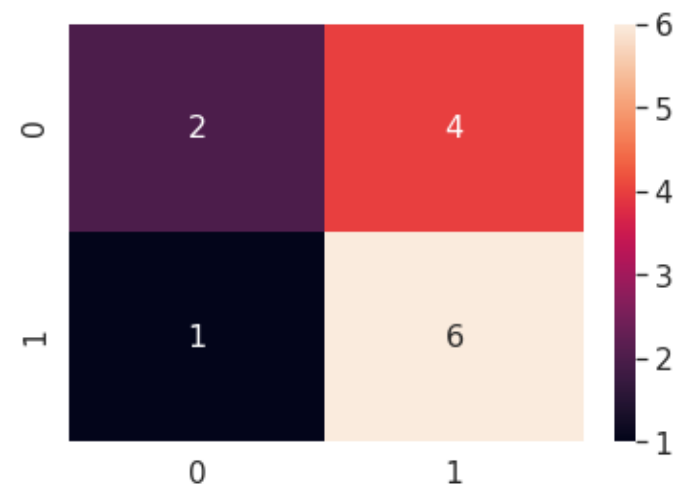
\includegraphics[width=0.9\textwidth]{images/resultados_lr_cm_conjunto1.png}
		\caption{Matriz de confusión para el modelo Regresión Logística en el caso de estudio 1.}
		\label{lrCMCase1}
	\end{subfigure}
	\begin{subfigure}[b]{0.45\linewidth} 
		\centering
	    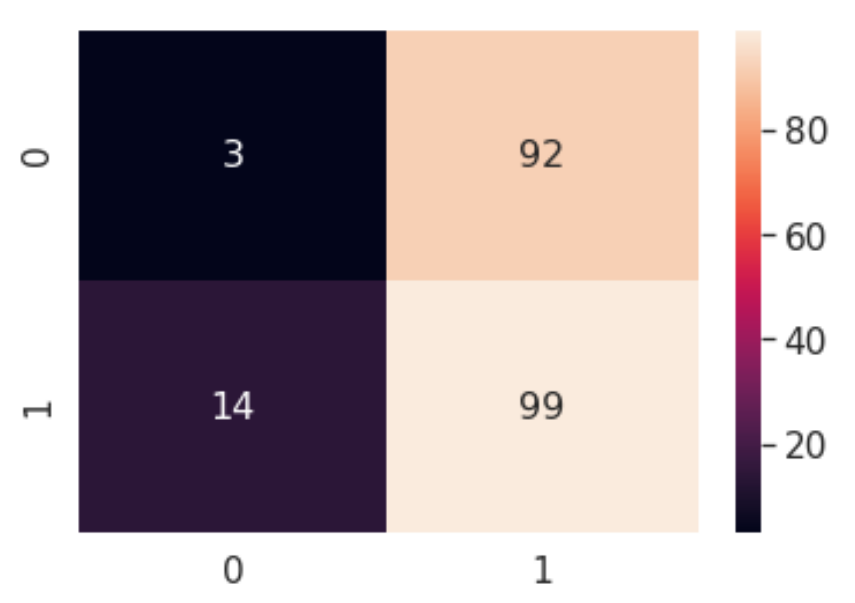
\includegraphics[width=0.9\textwidth]{images/resultados_lr_cm_conjunto2.png}
		\caption{Matriz de confusión para el modelo Regresión Logística en el caso de estudio 2.}
	  \label{lrCMCase2}
	\end{subfigure}
	\caption{Matriz de confusión para el modelo Regresión Logística.}
	\label{lrcm}
\end{figure}

\subsection{Conclusiones del modelo de Regresión Logística}
\label{resultados:lr_conclusiones}

\paragraph{}
Después de realizar el entrenamiento y posterior validación de los modelos podemos \textbf{desaconsejar su uso debido a su bajo porcentaje de aciertos}. Es posible que con un volumen de datos superior este se pueda comportar mejor, pero no se da el caso con el conjunto de datos que tenemos en la actualidad.

\section{Bosques Aleatorios '\textit{Random Forests}'.}
\label{resultados:rf}

\subsection{Características de los conjuntos de datos a analizar}
\label{resultados:rf_caracteristicas}
Al realizar las mismas transformaciones que para el caso de \hyperref[resultados:knn_caracteristicas]{K-NN}, las características de los conjuntos de datos son las mismas.

\subsection{(Caso de estudio 1) Resultados del entrenamiento con el Conjunto de datos solo con atributo utilidad definido y escogiendo los atributos que nos ha indicado como relevantes el \hyperref[result:pca_case2]{caso de estudio 2} del PCA}

\paragraph{}
Para realizar el entrenamiento y posterior validación del modelo de Bosques Aleatorios '\textit{Random Forests}' es necesario detectar antes a partir de que número de arboles podemos considerar que estos dan el valor a predecir correcto. Es lógico pensar que cuantos más arboles refuercen la decisión, más acertada sera esta pero, lo que hay que medir es, hasta que punto merece la pena seguir 'preguntando' si un registro es clasificado en un grupo u otro.

\paragraph{}
Esto es debido a que el modelo de Bosques Aleatorios '\textit{Random Forests}'\cite{ref:rf_def} genera versiones diferentes del conjunto de entrenamiento usando muestreo con reemplazo, usando la estrategia de \textit{bagging}\cite{ref:rf_bagging}. Esto significa que, durante el proceso de construcción de cada árbol de decisión, se selecciona aleatoriamente un subconjunto de las variables del conjunto de datos, dando opciones a variables que normalmente quedarían eclipsadas por otras que tengan mayor relevancia. Al tener un conjunto de datos con muy pocos atributos, tener un número elevado de arboles a preguntar hará que muchas veces se pregunte a arboles repetidos por lo que hay que valorar hasta que punto merece la pena seguir preguntando.

\paragraph{}
Para realizar este estudio ejecutaremos el modelo con diferentes valores de la variable \textit{n\_estimators}\cite{ref:rf_random_forest_classifier} (número de arboles en el bosque) y contrastaremos que porcentaje de acierto tiene el modelo con un subconjunto del propio conjunto de datos que conocemos su valor final. Como podemos ver en la figura \ref{rfTrainCase1}, el valor más optimo del \textbf{estimador es 40}, con un \textbf{porcentaje de acierto del 61\%}.

\paragraph{}
Si mostramos la matriz de confusión\cite{ref:confusion_matrix} (figura \ref{rfCMCase1}) para poder ver que porcentaje de aciertos tiene el modelo con el conjunto de test, vemos que tiene un porcentaje de aciertos bastante bajo llegando a rozar la aleatoriedad.

\begin{figure}[!htb]
    \begin{subfigure}[b]{0.45\linewidth}
    	\centering
	    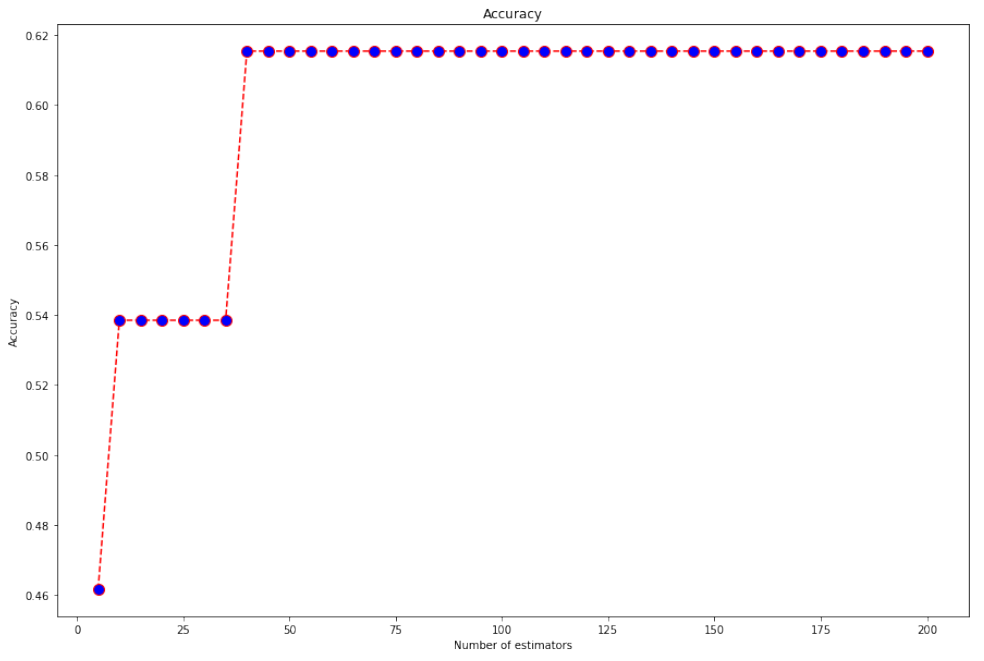
\includegraphics[width=0.9\textwidth]{images/resultados_rf_ent_conjunto1.png}
    	\caption{Calculo del valor n\_estimators para el caso de estudio 1.}
		\label{rfTrainCase1}
	\end{subfigure}
	\begin{subfigure}[b]{0.45\linewidth} 
		\centering
		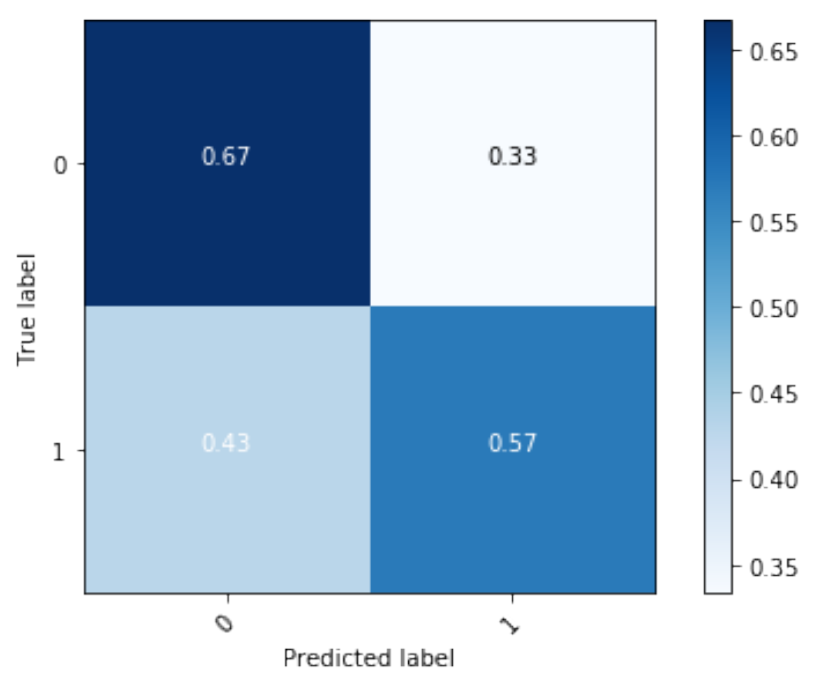
\includegraphics[width=0.7\textwidth]{images/resultados_rf_cm_conjunto1.png}
		\caption{Matriz de confusión para el modelo Random Forest en el caso de estudio 1.}
		\label{rfCMCase1}
	\end{subfigure}
	\caption{Modelo Random Forest en el caso de estudio 1.}
	\label{rfCase1}
\end{figure}

\subsection{(Caso de estudio 2) Conjunto de datos solo con atributo utilidad definido, añadiendo el mes y año del artículo, eliminando los atributos \textit{gender} y artículo y expandiendo el atributo \textit{respuesta.pubmed\_keys}. También escogemos solo los atributos que nos ha indicado como relevantes el \hyperref[result:pca_case3]{caso de estudio 3} del PCA.}

\paragraph{}
Igual que en el caso anterior, realizaremos el estudio para detectar a partir de que número de \textit{n\_estimators}\cite{ref:rf_random_forest_classifier} (número de arboles en el bosque) podemos dar por supuesto que el resultado es de un grupo u otro. A diferencia del caso anterior, podemos ver en la figura \ref{rfTrainCase2}, el valor más optimo del \textbf{estimador es 10}, con un \textbf{porcentaje de acierto del 89\%}.

\paragraph{}
Si mostramos la matriz de confusión\cite{ref:confusion_matrix} (figura \ref{rfCMCase2}) para poder ver que porcentaje de aciertos tiene el modelo con el conjunto de test, vemos que tiene un porcentaje de aciertos bastante aceptable.

\begin{figure}[!htb]
    \begin{subfigure}[b]{0.45\linewidth}
    	\centering
	    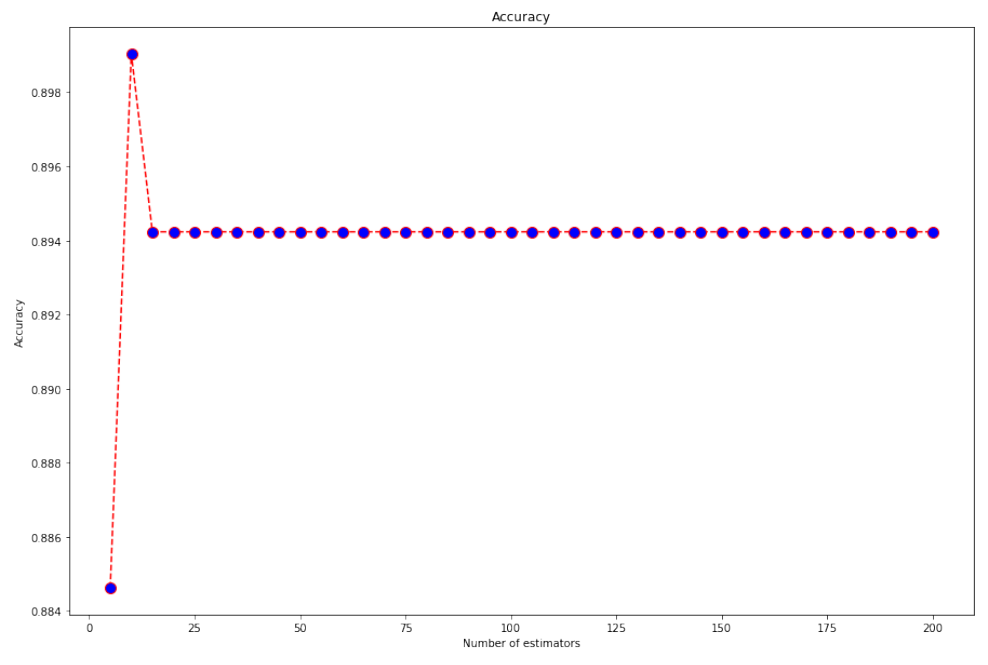
\includegraphics[width=0.9\textwidth]{images/resultados_rf_ent_conjunto2.png}
    	\caption{Calculo del valor n\_estimators para el caso de estudio 2.}
		\label{rfTrainCase2}
	\end{subfigure}
	\begin{subfigure}[b]{0.45\linewidth} 
		\centering
		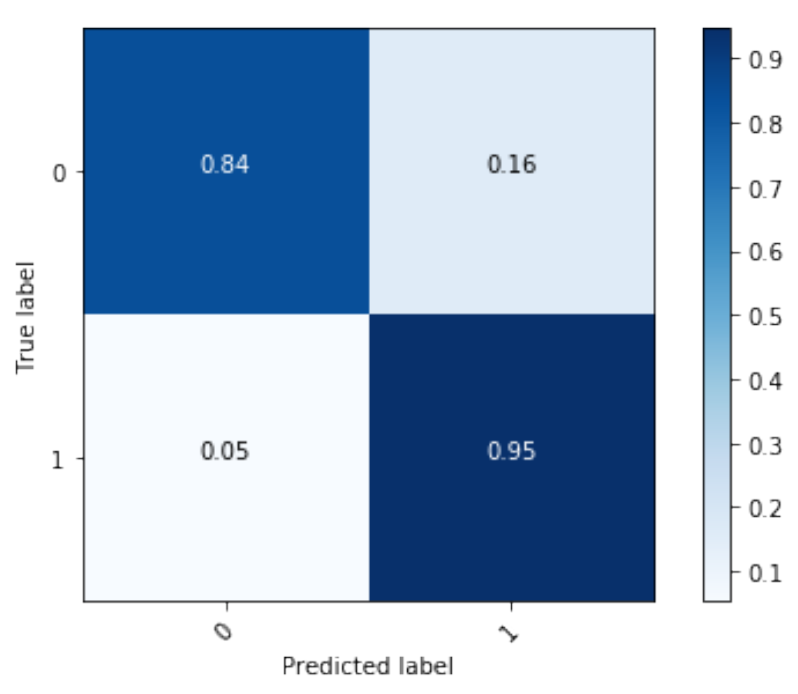
\includegraphics[width=0.7\textwidth]{images/resultados_rf_cm_conjunto2.png}
		\caption{Matriz de confusión para el modelo Random Forest en el caso de estudio 2.}
		\label{rfCMCase2}
	\end{subfigure}
	\caption{Modelo Random Forest en el caso de estudio 2.}
	\label{rfCase2}
\end{figure}

\subsection{Conclusiones del modelo de Regresión Logística}
\label{resultados:rf_conclusiones}

\paragraph{}
En este caso, podemos apreciar que el caso 2 se ajusta a unos resultados aceptables ya que esta lo suficientemente ajustado para que de resultados razonables si estar sobreajustado\cite{ref:knn_overfiting}. Por lo que recomendamos al cliente como posible modelo final el modelo de Bosques Aleatorios '\textit{Random Forests}' aplicando las transformaciones al conjunto de datos aplicados en el caso de estudio 2.

\newpage
\chapter{Conclusiones}
\label{chapter:conclusiones}

\section{Objetivos Secundarios}

\paragraph{}
En el apartado \nameref{section:analisis_datos} \textbf{se ha cumplido} el \hyperref[os:OS1]{OS1}, aplicado las transformaciones necesarias a los datos que tenemos para poder trabajar posteriormente con ellos con los modelos predictivos.

\paragraph{}
En el apartado \nameref{section:pca} \textbf{se ha cumplido} el \hyperref[os:OS2]{OS2}, pudiendo observar en el apartado de \hyperref[resultados:pca]{resultados}, que hay mucha diferencia según si se usa todas las observaciones o solo las que tienen informado el atributo a predecir (\textit{utilidad}), por lo que se decide junto con el cliente, intentar enriquecer los datos que no tienen informado el atributo (\textit{utilidad}) definiendo este paso como objetivo secundario \hyperref[os:OS3]{OS3}. Se analizara en el siguiente paso si el resultado de intentar enriquecer estos datos aporta algo al conjunto de datos.

\paragraph{}
En el apartado \nameref{section:knn} \textbf{no se ha podido cumplir} el \hyperref[os:OS3]{OS3}, pudiendo observar en el apartado de \hyperref[resultados:knn_conclusiones]{resultados} que el dataset se encuentra \hyperref[resultados:knn]{sesgado}, por lo que intentar enriquecer los datos lo único que generaría son falsos positivos, perjudicando a los posteriores entrenamientos de modelos predictivos que se estudian en este documento.

\paragraph{}
En el apartado \nameref{section:lr} \textbf{se ha cumplido} el \hyperref[os:OS4]{OS4}, realizando el estudio de la aplicación del modelo de Regresión Logística, pudiendo observar su \hyperref[resultados:lr]{bajo nivel de precisión}, llegando a desaconsejar su uso con el conjunto de datos actual.

\paragraph{}
En el apartado \nameref{section:rf} \textbf{se ha cumplido} el \hyperref[os:OS5]{OS5}, realizando el estudio de la aplicación del modelo de Bosques Aleatorios '\textit{Random Forests}, pudiendo observar \hyperref[resultados:rf]{un nivel de precisión aceptable para el caso de estudio 2}, llegando a aconsejar su uso con el conjunto de datos actual.
\newpage
\chapter{Anexos}
\label{chapter:anexos}


\section{Procesado de datos}
\label{anx01:procesado_datos}
\href{file://./anexos/S0 - HOPE extract data.pdf}{S0 - HOPE extract data.pdf}

\section{Análisis de componentes principales}
\label{anx02:pca}
\subsection{Iteración 1}
\label{anx02:pca1}
\href{file://./anexos/S1 - HOPE PCA.pdf}{S1 - HOPE PCA.pdf}

\subsection{Iteración 2}
\label{anx02:pca2}
\href{file://./anexos/S1 - HOPE PCA_v2.pdf}{S1 - HOPE PCA\_v2.pdf}

\subsection{Iteración 3}
\label{anx02:pca3}
\href{file://./anexos/S1 - HOPE PCA_v3.pdf}{S1 - HOPE PCA\_v3.pdf}


\newpage

% bibliografia
\addcontentsline{toc}{chapter}{Bibliografía}
\bibliography{referencias}
\bibliographystyle{ieeetr}


\end{document}